% Edit only the text between matching begin and end lines.
\documentclass[11pt,a4paper]{article}
% Shared preamble for TMUA question papers. Local edits here are overwritten.

% Reproducible PDFs: no timestamps, no trailer id, no build-path details.
\ifdefined\pdfsuppressptexinfo
  \pdfsuppressptexinfo=-1
  \pdfinfoomitdate=1
  \pdftrailerid{}
\fi

\usepackage{graphicx}
\usepackage{mathtools}
\usepackage{amssymb}
\usepackage{amsmath}
\usepackage{amsthm}
\usepackage{enumitem}
\usepackage{microtype}
\usepackage[table]{xcolor}
\usepackage{array}
\usepackage{booktabs}
\usepackage{tabularx}
\usepackage{longtable}
\usepackage{ragged2e}
\usepackage{fancyhdr}
\usepackage{etoolbox}
\usepackage[
  a4paper,
  left=0.8in,
  right=1in,
  top=1in,
  bottom=0.5in,
  headheight=14pt,
  headsep=0.4in
]{geometry}

\usepackage{pgfplots}
\pgfplotsset{compat=1.18}
\usepgfplotslibrary{fillbetween, polar}
\usetikzlibrary{calc, positioning}
\usetikzlibrary{angles, quotes}
\usetikzlibrary{arrows.meta}
\usetikzlibrary{decorations.pathreplacing, decorations.markings}
\usetikzlibrary{patterns}
\usetikzlibrary{intersections}

\usepackage{tocloft}
\usepackage[hidelinks]{hyperref}
\hypersetup{pdfauthor={danieljsmith.org}, pdfcreator={}, pdfsubject={}, pdfkeywords={}}
\urlstyle{same}
\tocloftpagestyle{djspaper}
\setlength{\cftbeforesubsecskip}{2pt}
\setlength{\cftsubsecindent}{1.5em}
\setlength{\cftsubsecnumwidth}{0pt}
\renewcommand{\cftsubsecfont}{\small\color{black}}
\renewcommand{\cftsubsecpagefont}{\small\color{black}}
\renewcommand{\cftsubsecleader}{\hfill}

% \djsPaperSetup{<PDF title>}{<header label>}, called once after this file.
\newcommand{\djsHeaderLabel}{}
\newcommand{\djsPaperSetup}[2]{%
  \hypersetup{pdftitle={#1}}%
  \renewcommand{\djsHeaderLabel}{#2}}

\setlength{\parindent}{0pt}
\fancypagestyle{djspaper}{%
  \fancyhead{}%
  \fancyfoot{}%
  \renewcommand{\headrulewidth}{0.9pt}%
  \fancyhead[L]{\djsHeaderLabel}%
  \fancyhead[R]{\href{https://danieljsmith.org}{danieljsmith.org}}%
}
\pagestyle{djspaper}

\newcolumntype{Y}{>{\RaggedRight\arraybackslash}X}

% Topic labels: a subtle line above each question and a suffix on its
% contents entry. The bookmark form is spelled out separately, because a PDF
% bookmark is plain text and would otherwise keep the colour name.
\newcommand{\djsTocTopic}[1]{%
  \ifblank{#1}{}{%
    \texorpdfstring
      {\hspace{0.9em}{\footnotesize\itshape\color{black!45}#1}}
      { \textendash\ #1}}}
\newcommand{\djsTopicLine}[1]{%
  \ifblank{#1}{}{%
    {\raggedleft\footnotesize\itshape\color{black!45}#1\par}%
    \vspace{-0.6\baselineskip}}}

\newcommand{\questionitem}[1][]{%
  \item\phantomsection
  \addcontentsline{toc}{subsection}{%
    Question \number\value{enumi}\protect\djsTocTopic{#1}}%
}
\renewcommand{\contentsname}{Questions}
\newcommand{\djsFrontMatter}{%
  \vspace*{20pt}%
  \tableofcontents
  \newpage
}

\djsPaperSetup{TMUA Set B Paper 1}{TMUA Set B - Paper 1}
\begin{document}
\thispagestyle{djspaper}
\djsFrontMatter
\thispagestyle{djspaper}
\vspace*{8pt}
\djsTopicLine{Sequences \& Series}
\begin{enumerate}[label=\textbf{\arabic*.},leftmargin=*,itemsep=0pt,start=1]
\questionitem[Sequences \& Series]
% begin q000675 stem
An infinite geometric series has first term $a$ and common ratio $r$.

The sum to infinity of this series is $S$.

The sum to infinity of the squares of the terms of this series is $2S$.

The sum to infinity of the cubes of the terms of this series is $\dfrac{36}{7}S$.

What is the value of $S$?
% end q000675 stem

\par\vspace*{12pt}
\begin{tabularx}{\linewidth}{@{}>{\bfseries}l Y@{}}
A &
% begin q000675 choice A
$2$
% end q000675 choice A
\\[0.8em]
B &
% begin q000675 choice B
$3$
% end q000675 choice B
\\[0.8em]
C &
% begin q000675 choice C
$4$
% end q000675 choice C
\\[0.8em]
D &
% begin q000675 choice D
$6$
% end q000675 choice D
\\[0.8em]
E &
% begin q000675 choice E
$8$
% end q000675 choice E
\\[0.8em]
F &
% begin q000675 choice F
$9$
% end q000675 choice F
\\[0.8em]
G &
% begin q000675 choice G
$12$
% end q000675 choice G
\\
\end{tabularx}
\end{enumerate}
\clearpage
\thispagestyle{djspaper}
\vspace*{8pt}
\djsTopicLine{Algebra}
\begin{enumerate}[label=\textbf{\arabic*.},leftmargin=*,itemsep=0pt,start=2]
\questionitem[Algebra]
% begin q000599 stem
A straight line with gradient $m$ passes through the point $(1, 4)$

The line intersects the curve $y = x^2$ at two distinct points with $x$-coordinates $x_1$ and $x_2$

What is the minimum possible value of $x_1^2 + x_2^2$ as $m$ varies over all real numbers?
% end q000599 stem

\par\vspace*{12pt}
\begin{tabularx}{\linewidth}{@{}>{\bfseries}l Y@{}}
A &
% begin q000599 choice A
$1$
% end q000599 choice A
\\[0.8em]
B &
% begin q000599 choice B
$4$
% end q000599 choice B
\\[0.8em]
C &
% begin q000599 choice C
$7$
% end q000599 choice C
\\[0.8em]
D &
% begin q000599 choice D
$8$
% end q000599 choice D
\\[0.8em]
E &
% begin q000599 choice E
$12$
% end q000599 choice E
\\[0.8em]
F &
% begin q000599 choice F
$16$
% end q000599 choice F
\\
\end{tabularx}
\end{enumerate}
\clearpage
\thispagestyle{djspaper}
\vspace*{8pt}
\djsTopicLine{Trigonometry}
\begin{enumerate}[label=\textbf{\arabic*.},leftmargin=*,itemsep=0pt,start=3]
\questionitem[Trigonometry]
% begin q000073 stem
Let \(n\) be a positive integer.

Suppose that
\[
\sum_{k=0}^{n-1}\cos\!\left(\theta+\frac{k\pi}{2}\right)=0
\]
for every real value of \(\theta\).

Which of the following is the complete set of possible values of \(n\)?
% end q000073 stem

\par\vspace*{12pt}
\begin{tabularx}{\linewidth}{@{}>{\bfseries}l Y@{}}
A &
% begin q000073 choice A
$n$ is odd
% end q000073 choice A
\\[0.8em]
B &
% begin q000073 choice B
$n$ is even
% end q000073 choice B
\\[0.8em]
C &
% begin q000073 choice C
$n$ is a multiple of 3
% end q000073 choice C
\\[0.8em]
D &
% begin q000073 choice D
$n$ is a multiple of 4
% end q000073 choice D
\\[0.8em]
E &
% begin q000073 choice E
$n$ is 1 more than a multiple of 4
% end q000073 choice E
\\[0.8em]
F &
% begin q000073 choice F
$n$ is 2 more than a multiple of 4
% end q000073 choice F
\\
\end{tabularx}
\end{enumerate}
\clearpage
\thispagestyle{djspaper}
\vspace*{8pt}
\djsTopicLine{Exponentials \& Logarithms}
\begin{enumerate}[label=\textbf{\arabic*.},leftmargin=*,itemsep=0pt,start=4]
\questionitem[Exponentials \& Logarithms]
% begin q000056 stem
For real parameter $t$, consider the equation \[ \log_3 x + \log_x 3 = t \] with $x>0$ and $x\ne 1$.

The number of positive solutions $x$ is
% end q000056 stem

\par\vspace*{12pt}
\begin{tabularx}{\linewidth}{@{}>{\bfseries}l Y@{}}
A &
% begin q000056 choice A
two if $|t|>2$, one if $|t|=2$, and zero if $|t|<2$
% end q000056 choice A
\\[0.8em]
B &
% begin q000056 choice B
one if $t>0$, and zero if $t<0$
% end q000056 choice B
\\[0.8em]
C &
% begin q000056 choice C
zero if $t>2$, one if $t=2$, and two if $0<t<2$
% end q000056 choice C
\\[0.8em]
D &
% begin q000056 choice D
one for all real $t$
% end q000056 choice D
\\[0.8em]
E &
% begin q000056 choice E
two if $t<-2$, zero if $t>-2$, and one if $t=-2$
% end q000056 choice E
\\
\end{tabularx}
\end{enumerate}
\clearpage
\thispagestyle{djspaper}
\vspace*{8pt}
\djsTopicLine{Coordinate Geometry}
\begin{enumerate}[label=\textbf{\arabic*.},leftmargin=*,itemsep=0pt,start=5]
\questionitem[Coordinate Geometry]
% begin q000661 stem
The points $A$ and $B$ have coordinates $(0,0)$ and $(10,0)$ respectively. 

A circle has diameter $AB$.

The point $C$ lies on the circle above the $x$-axis, with $AC=6$ and $BC=8$.

The tangent to the circle at $C$ meets the lines $x=0$ and $x=10$ at $P$ and $Q$ respectively.

What is the length $PQ$?
% end q000661 stem

\begin{center}
% begin q000661 diagram
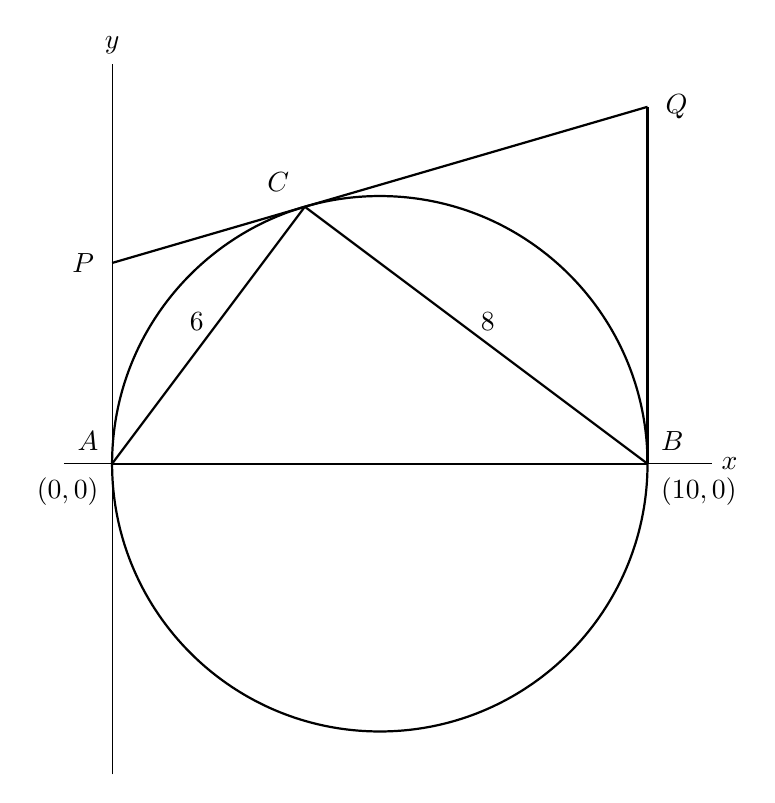
\begin{tikzpicture}[x=0.68cm,y=0.68cm]
\def\ABlen{10}
\pgfmathsetmacro{\rad}{\ABlen/2}
\pgfmathsetmacro{\Ox}{\ABlen/2}
\pgfmathsetmacro{\Cx}{18/5}
\pgfmathsetmacro{\Cy}{24/5}
\pgfmathsetmacro{\Py}{15/4}
\pgfmathsetmacro{\Qy}{20/3}
\pgfmathsetmacro{\xmin}{-0.9}
\pgfmathsetmacro{\xmax}{\ABlen+1.2}
\pgfmathsetmacro{\ymin}{-\rad-0.8}
\pgfmathsetmacro{\ymax}{\Qy+0.8}

\coordinate (A) at (0,0);
\coordinate (B) at (\ABlen,0);
\coordinate (O) at (\Ox,0);
\coordinate (C) at (\Cx,\Cy);
\coordinate (P) at (0,\Py);
\coordinate (Q) at (\ABlen,\Qy);

% Coordinate axes
\draw[black] (\xmin,0) -- (\xmax,0) node[right] {$x$};
\draw[black] (0,\ymin) -- (0,\ymax) node[above] {$y$};

% Circle and geometric segments
\draw[thick,black] (O) circle (\rad);
\draw[thick,black] (A) -- (B);
\draw[thick,black] (A) -- (C)
    node[midway,above left, yshift=-2pt, xshift=2pt] {$6$};
\draw[thick,black] (C) -- (B)
    node[midway,above right, yshift=-2pt, xshift=-2pt] {$8$};
\draw[thick,black] (P) -- (Q);
\draw[thick,black] (B) -- (Q);

% Point and coordinate labels
\node[above left=2pt] at (A) {$A$};
\node[below left=2pt] at (A) {$(0,0)$};
\node[above right=2pt] at (B) {$B$};
\node[below right=2pt] at (B) {$(10,0)$};
\node[above left=3pt] at (C) {$C$};
\node[left=3pt] at (P) {$P$};
\node[right=3pt] at (Q) {$Q$};
\end{tikzpicture}
% end q000661 diagram
\end{center}

\par\vspace*{12pt}
\begin{tabularx}{\linewidth}{@{}>{\bfseries}l Y@{}}
A &
% begin q000661 choice A
$\dfrac{35}{12}$
% end q000661 choice A
\\[0.8em]
B &
% begin q000661 choice B
$\dfrac{15}{4}$
% end q000661 choice B
\\[0.8em]
C &
% begin q000661 choice C
$\dfrac{20}{3}$
% end q000661 choice C
\\[0.8em]
D &
% begin q000661 choice D
$10$
% end q000661 choice D
\\[0.8em]
E &
% begin q000661 choice E
$\dfrac{125}{12}$
% end q000661 choice E
\\[0.8em]
F &
% begin q000661 choice F
$\dfrac{125}{6}$
% end q000661 choice F
\\
\end{tabularx}
\end{enumerate}
\clearpage
\thispagestyle{djspaper}
\vspace*{8pt}
\djsTopicLine{Integration}
\begin{enumerate}[label=\textbf{\arabic*.},leftmargin=*,itemsep=0pt,start=6]
\questionitem[Integration]
% begin q000611 stem
Let $k$ be a positive real constant. The function $f(x)$ is defined for $x > 0$ by

\[ f(x) = \int_1^x \frac{t - k}{\sqrt{t}} \, \mathrm{d}t \]

What is the complete set of values of $k$ for which the equation $f(x) = 0$ has exactly two distinct real solutions for $x > 0$?
% end q000611 stem

\par\vspace*{12pt}
\begin{tabularx}{\linewidth}{@{}>{\bfseries}l Y@{}}
A &
% begin q000611 choice A
$k > 1$
% end q000611 choice A
\\[0.8em]
B &
% begin q000611 choice B
$k > \frac{1}{3}$
% end q000611 choice B
\\[0.8em]
C &
% begin q000611 choice C
$k > \frac{1}{3}$ and $k \neq 1$
% end q000611 choice C
\\[0.8em]
D &
% begin q000611 choice D
$\frac{1}{3} < k < 1$
% end q000611 choice D
\\[0.8em]
E &
% begin q000611 choice E
$k > 0$ and $k \neq 1$
% end q000611 choice E
\\[0.8em]
F &
% begin q000611 choice F
$k \ge \frac{1}{4}$ and $k \neq 1$
% end q000611 choice F
\\
\end{tabularx}
\end{enumerate}
\clearpage
\thispagestyle{djspaper}
\vspace*{8pt}
\djsTopicLine{Geometry}
\begin{enumerate}[label=\textbf{\arabic*.},leftmargin=*,itemsep=0pt,start=7]
\questionitem[Geometry]
% begin q000055 stem
In triangle $ABC$, $AB=9$, $\angle ABC=30^\circ$, and $AC=x$, where $x>0$.

For which values of $x$ is there exactly one possible length of $BC$?
% end q000055 stem

\par\vspace*{12pt}
\begin{tabularx}{\linewidth}{@{}>{\bfseries}l Y@{}}
A &
% begin q000055 choice A
$x<\frac{9}{2}$
% end q000055 choice A
\\[0.8em]
B &
% begin q000055 choice B
$x=\frac{9}{2}$ or $x\ge 9$
% end q000055 choice B
\\[0.8em]
C &
% begin q000055 choice C
$\frac{9}{2}<x<9$
% end q000055 choice C
\\[0.8em]
D &
% begin q000055 choice D
$x\ge\frac{9}{2}$
% end q000055 choice D
\\[0.8em]
E &
% begin q000055 choice E
$x=9$ only
% end q000055 choice E
\\[0.8em]
F &
% begin q000055 choice F
$x>0$
% end q000055 choice F
\\[0.8em]
G &
% begin q000055 choice G
$0<x<\frac{9}{2}$ or $x>9$
% end q000055 choice G
\\
\end{tabularx}
\end{enumerate}
\clearpage
\thispagestyle{djspaper}
\vspace*{8pt}
\djsTopicLine{Probability \& Counting}
\begin{enumerate}[label=\textbf{\arabic*.},leftmargin=*,itemsep=0pt,start=8]
\questionitem[Probability \& Counting]
% begin q000562 stem
$N=2^7 \times 3^5$

One of the positive factors of $N$ that is divisible by $12$ is selected at random, with each such factor equally likely to be selected.

What is the probability that $N$ divided by the selected factor is a perfect square?
% end q000562 stem

\par\vspace*{12pt}
\begin{tabularx}{\linewidth}{@{}>{\bfseries}l Y@{}}
A &
% begin q000562 choice A
$\dfrac{1}{6}$
% end q000562 choice A
\\[0.8em]
B &
% begin q000562 choice B
$\dfrac{1}{5}$
% end q000562 choice B
\\[0.8em]
C &
% begin q000562 choice C
$\dfrac{1}{4}$
% end q000562 choice C
\\[0.8em]
D &
% begin q000562 choice D
$\dfrac{3}{10}$
% end q000562 choice D
\\[0.8em]
E &
% begin q000562 choice E
$\dfrac{1}{3}$
% end q000562 choice E
\\[0.8em]
F &
% begin q000562 choice F
$\dfrac{2}{5}$
% end q000562 choice F
\\
\end{tabularx}
\end{enumerate}
\clearpage
\thispagestyle{djspaper}
\vspace*{8pt}
\djsTopicLine{Geometry}
\begin{enumerate}[label=\textbf{\arabic*.},leftmargin=*,itemsep=0pt,start=9]
\questionitem[Geometry]
% begin q000623 stem
The diagram shows a semicircle of radius $1$ with its diameter along the $x$-axis and its centre at the origin.

A rectangle has one side on the diameter and its two remaining vertices on the arc of the semicircle.

What is the largest possible perimeter of such a rectangle?
% end q000623 stem

\begin{center}
% begin q000623 diagram
\begin{tikzpicture}[scale=4]
\def\xmin{-1.4}
\def\xmax{1.4}
\def\ymin{-0.3}
\def\ymax{1.3}
\def\radius{1}
\def\xrect{0.62}
\pgfmathsetmacro{\hrect}{sqrt(\radius^2-\xrect^2)}

\coordinate (O) at (0,0);
\coordinate (L) at (-\radius,0);
\coordinate (R) at (\radius,0);
\coordinate (A) at (-\xrect,0);
\coordinate (B) at (\xrect,0);
\coordinate (C) at (\xrect,\hrect);
\coordinate (D) at (-\xrect,\hrect);
\coordinate (Q) at (45:\radius);

\draw[->] (\xmin,0) -- (\xmax,0) node[right] {$x$};
\draw[->] (0,\ymin) -- (0,\ymax) node[above] {$y$};

\draw[thick, black] (L) arc[start angle=180,end angle=0,radius=\radius];
\draw[thick, black] (L) -- (R);
\draw[thick, black] (A) -- (B) -- (C) -- (D) -- cycle;

\node[below left] at (O) {$O$};
\end{tikzpicture}
% end q000623 diagram
\end{center}

\par\vspace*{12pt}
\begin{tabularx}{\linewidth}{@{}>{\bfseries}l Y@{}}
A &
% begin q000623 choice A
$\sqrt{5}$
% end q000623 choice A
\\[0.8em]
B &
% begin q000623 choice B
$4$
% end q000623 choice B
\\[0.8em]
C &
% begin q000623 choice C
$2+\sqrt{5}$
% end q000623 choice C
\\[0.8em]
D &
% begin q000623 choice D
$3\sqrt{2}$
% end q000623 choice D
\\[0.8em]
E &
% begin q000623 choice E
$2\sqrt{5}$
% end q000623 choice E
\\[0.8em]
F &
% begin q000623 choice F
$5$
% end q000623 choice F
\\
\end{tabularx}
\end{enumerate}
\clearpage
\thispagestyle{djspaper}
\vspace*{8pt}
\djsTopicLine{Trigonometry}
\begin{enumerate}[label=\textbf{\arabic*.},leftmargin=*,itemsep=0pt,start=10]
\questionitem[Trigonometry]
% begin q000618 stem
Consider the equation
\[ \sin^2 x - (2k-1)\sin x + k^2 - k = 0 \]
where $k$ is a real constant.

Find the complete set of values of $k$ for which the equation has exactly three distinct real solutions in the range $0 \le x < 2\pi$.
% end q000618 stem

\par\vspace*{12pt}
\begin{tabularx}{\linewidth}{@{}>{\bfseries}l Y@{}}
A &
% begin q000618 choice A
$k = 0$ or $k = 1$
% end q000618 choice A
\\[0.8em]
B &
% begin q000618 choice B
$k = -1$ or $k = 2$
% end q000618 choice B
\\[0.8em]
C &
% begin q000618 choice C
$k = -1$, $k = 0$, $k = 1$, or $k = 2$
% end q000618 choice C
\\[0.8em]
D &
% begin q000618 choice D
$0 < k < 1$
% end q000618 choice D
\\[0.8em]
E &
% begin q000618 choice E
$-1 < k < 0$ or $1 < k < 2$
% end q000618 choice E
\\[0.8em]
F &
% begin q000618 choice F
$-1 < k < 1$
% end q000618 choice F
\\[0.8em]
G &
% begin q000618 choice G
$-1 \le k \le 1$
% end q000618 choice G
\\[0.8em]
H &
% begin q000618 choice H
There are no values of $k$.
% end q000618 choice H
\\
\end{tabularx}
\end{enumerate}
\clearpage
\thispagestyle{djspaper}
\vspace*{8pt}
\djsTopicLine{Sequences \& Series}
\begin{enumerate}[label=\textbf{\arabic*.},leftmargin=*,itemsep=0pt,start=11]
\questionitem[Sequences \& Series]
% begin q000037 stem
A sequence $a_n$ is defined by $a_1=1$ and, for $n\ge 1$, \[ a_{n+1}=a_n+\dfrac{1}{a_n} \] Which of the following statements is true for all $n\ge 1$?
% end q000037 stem

\par\vspace*{12pt}
\begin{tabularx}{\linewidth}{@{}>{\bfseries}l Y@{}}
A &
% begin q000037 choice A
$a_n$ is an integer
% end q000037 choice A
\\[0.8em]
B &
% begin q000037 choice B
$a_n^2$ is an integer
% end q000037 choice B
\\[0.8em]
C &
% begin q000037 choice C
$a_n<n$
% end q000037 choice C
\\[0.8em]
D &
% begin q000037 choice D
$a_n^2 \ge 2n-1$
% end q000037 choice D
\\[0.8em]
E &
% begin q000037 choice E
$a_n^2 \le 2n-1$
% end q000037 choice E
\\[0.8em]
F &
% begin q000037 choice F
$a_n \le \sqrt{2n}$
% end q000037 choice F
\\
\end{tabularx}
\end{enumerate}
\clearpage
\thispagestyle{djspaper}
\vspace*{8pt}
\djsTopicLine{Number}
\begin{enumerate}[label=\textbf{\arabic*.},leftmargin=*,itemsep=0pt,start=12]
\questionitem[Number]
% begin q000165 stem
The positive real numbers $p \times 10^{-4}$, $q \times 10^{-2}$ and $r \times 10^{-1}$ are each in standard form, and \[ (p \times 10^{-4}) + (q \times 10^{-2}) = (r \times 10^{-1}) \] \textit{How many} of the following statements must be true? \[ \begin{array}{@{}l l@{}}
\textbf{I:} & \text{$q>1$} \\[2pt]
\textbf{II:} & \text{$r>1$} \\[2pt]
\textbf{III:} & \text{$q<r$} \\[2pt]
\textbf{IV:} & \text{$p<r$}
\end{array} \]
% end q000165 stem

\par\vspace*{12pt}
\begin{tabularx}{\linewidth}{@{}>{\bfseries}l Y@{}}
A &
% begin q000165 choice A
1 of them
% end q000165 choice A
\\[0.8em]
B &
% begin q000165 choice B
2 of them
% end q000165 choice B
\\[0.8em]
C &
% begin q000165 choice C
3 of them
% end q000165 choice C
\\[0.8em]
D &
% begin q000165 choice D
4 of them
% end q000165 choice D
\\[0.8em]
E &
% begin q000165 choice E
None of them
% end q000165 choice E
\\
\end{tabularx}
\end{enumerate}
\clearpage
\thispagestyle{djspaper}
\vspace*{8pt}
\djsTopicLine{Probability \& Counting}
\begin{enumerate}[label=\textbf{\arabic*.},leftmargin=*,itemsep=0pt,start=13]
\questionitem[Probability \& Counting]
% begin q000566 stem
A bag contains only red balls and blue balls, with at least one ball of each colour. The total number of balls is $n$, where $30<n<50$.

Two balls are drawn at random without replacement. The probability that they have the same colour is equal to the probability that they have different colours.

How many different possible values are there for the number of red balls in the bag?
% end q000566 stem

\par\vspace*{12pt}
\begin{tabularx}{\linewidth}{@{}>{\bfseries}l Y@{}}
A &
% begin q000566 choice A
$1$
% end q000566 choice A
\\[0.8em]
B &
% begin q000566 choice B
$2$
% end q000566 choice B
\\[0.8em]
C &
% begin q000566 choice C
$3$
% end q000566 choice C
\\[0.8em]
D &
% begin q000566 choice D
$4$
% end q000566 choice D
\\[0.8em]
E &
% begin q000566 choice E
$5$
% end q000566 choice E
\\
\end{tabularx}
\end{enumerate}
\clearpage
\thispagestyle{djspaper}
\vspace*{8pt}
\djsTopicLine{Inequalities}
\begin{enumerate}[label=\textbf{\arabic*.},leftmargin=*,itemsep=0pt,start=14]
\questionitem[Inequalities]
% begin q000039 stem
In this question, $a_1, \ldots, a_{50}$ and $b_1, \ldots, b_{50}$ are real numbers such that \[ a_n \le 2 b_n + 5 \] for each $n$ Consider the following statements: \[ \begin{array}{@{}l l@{}}
\textbf{I:} & \text{(minimum of $a_1,\ldots,a_{50}$) $\le 2\times$ (minimum of $b_1,\ldots,b_{50}$) $+\,5$} \\[2pt]
\textbf{II:} & \text{(maximum of $a_1,\ldots,a_{50}$) $\le 2\times$ (maximum of $b_1,\ldots,b_{50}$) $+\,5$} \\[2pt]
\textbf{III:} & \text{(minimum of $a_1,\ldots,a_{50}$) $\ge 2\times$ (minimum of $b_1,\ldots,b_{50}$) $+\,5$}
\end{array} \] Which of these statements must be true?
% end q000039 stem

\par\vspace*{12pt}
\begin{tabularx}{\linewidth}{@{}>{\bfseries}l Y@{}}
A &
% begin q000039 choice A
None of them
% end q000039 choice A
\\[0.8em]
B &
% begin q000039 choice B
I only
% end q000039 choice B
\\[0.8em]
C &
% begin q000039 choice C
II only
% end q000039 choice C
\\[0.8em]
D &
% begin q000039 choice D
III only
% end q000039 choice D
\\[0.8em]
E &
% begin q000039 choice E
I and II only
% end q000039 choice E
\\[0.8em]
F &
% begin q000039 choice F
I and III only
% end q000039 choice F
\\[0.8em]
G &
% begin q000039 choice G
II and III only
% end q000039 choice G
\\[0.8em]
H &
% begin q000039 choice H
I, II and III
% end q000039 choice H
\\
\end{tabularx}
\end{enumerate}
\clearpage
\thispagestyle{djspaper}
\vspace*{8pt}
\djsTopicLine{Number}
\begin{enumerate}[label=\textbf{\arabic*.},leftmargin=*,itemsep=0pt,start=15]
\questionitem[Number]
% begin q000583 stem
Let $N=2^6\times3^4\times5^3$

A positive factor $d$ of $N$ is chosen such that the highest common factor of $d$ and $\frac{N}{d}$ is $60$.

How many possible values of $d$ are there?
% end q000583 stem

\par\vspace*{12pt}
\begin{tabularx}{\linewidth}{@{}>{\bfseries}l Y@{}}
A &
% begin q000583 choice A
$2$
% end q000583 choice A
\\[0.8em]
B &
% begin q000583 choice B
$4$
% end q000583 choice B
\\[0.8em]
C &
% begin q000583 choice C
$6$
% end q000583 choice C
\\[0.8em]
D &
% begin q000583 choice D
$8$
% end q000583 choice D
\\[0.8em]
E &
% begin q000583 choice E
$12$
% end q000583 choice E
\\
\end{tabularx}
\end{enumerate}
\clearpage
\thispagestyle{djspaper}
\vspace*{8pt}
\djsTopicLine{Polynomials}
\begin{enumerate}[label=\textbf{\arabic*.},leftmargin=*,itemsep=0pt,start=16]
\questionitem[Polynomials]
% begin q000072 stem
Consider
\[P(x)=x^4+ax^3+bx^2+ax+1\]
where $a$ and $b$ are real constants.

Suppose $(x-2)$ and $\left(x+\frac{1}{2}\right)$ are both factors of $P(x)$

What is the value of $b$?
% end q000072 stem

\par\vspace*{12pt}
\begin{tabularx}{\linewidth}{@{}>{\bfseries}l Y@{}}
A &
% begin q000072 choice A
$-13$
% end q000072 choice A
\\[0.8em]
B &
% begin q000072 choice B
$-5$
% end q000072 choice B
\\[0.8em]
C &
% begin q000072 choice C
$0$
% end q000072 choice C
\\[0.8em]
D &
% begin q000072 choice D
$5$
% end q000072 choice D
\\[0.8em]
E &
% begin q000072 choice E
$13$
% end q000072 choice E
\\[0.8em]
F &
% begin q000072 choice F
$-\frac{17}{4}$
% end q000072 choice F
\\
\end{tabularx}
\end{enumerate}
\clearpage
\thispagestyle{djspaper}
\vspace*{8pt}
\djsTopicLine{Integration}
\begin{enumerate}[label=\textbf{\arabic*.},leftmargin=*,itemsep=0pt,start=17]
\questionitem[Integration]
% begin q000614 stem
Let $k$ be a positive constant. The curve $C$ has equation \[y = x^3 - 3k^2 x + 2k^3\]
The point $A$ is the local maximum of $C$.

The line parallel to the $x$-axis passing through $A$ intersects $C$ again at the point $B$.

The area of the region bounded by $C$ and the line segment $AB$ is $108$.

What is the value of $k$?
% end q000614 stem

\par\vspace*{12pt}
\begin{tabularx}{\linewidth}{@{}>{\bfseries}l Y@{}}
A &
% begin q000614 choice A
$1$
% end q000614 choice A
\\[0.8em]
B &
% begin q000614 choice B
$\sqrt{2}$
% end q000614 choice B
\\[0.8em]
C &
% begin q000614 choice C
$\sqrt{3}$
% end q000614 choice C
\\[0.8em]
D &
% begin q000614 choice D
$2$
% end q000614 choice D
\\[0.8em]
E &
% begin q000614 choice E
$2\sqrt{2}$
% end q000614 choice E
\\[0.8em]
F &
% begin q000614 choice F
$3$
% end q000614 choice F
\\[0.8em]
G &
% begin q000614 choice G
$4$
% end q000614 choice G
\\
\end{tabularx}
\end{enumerate}
\clearpage
\thispagestyle{djspaper}
\vspace*{8pt}
\djsTopicLine{Algebra}
\begin{enumerate}[label=\textbf{\arabic*.},leftmargin=*,itemsep=0pt,start=18]
\questionitem[Algebra]
% begin q000135 stem
Let $a$ and $b$ be real numbers with $a+b=1$

What is the least possible value of \[(a^2 + b)(b^2 + a)\quad?\]
% end q000135 stem

\par\vspace*{12pt}
\begin{tabularx}{\linewidth}{@{}>{\bfseries}l Y@{}}
A &
% begin q000135 choice A
$\dfrac{9}{16}$
% end q000135 choice A
\\[0.8em]
B &
% begin q000135 choice B
$\dfrac{1}{4}$
% end q000135 choice B
\\[0.8em]
C &
% begin q000135 choice C
$\dfrac{1}{2}$
% end q000135 choice C
\\[0.8em]
D &
% begin q000135 choice D
$\dfrac{3}{4}$
% end q000135 choice D
\\[0.8em]
E &
% begin q000135 choice E
$1$
% end q000135 choice E
\\
\end{tabularx}
\end{enumerate}
\clearpage
\thispagestyle{djspaper}
\vspace*{8pt}
\djsTopicLine{Functions \& Graphs}
\begin{enumerate}[label=\textbf{\arabic*.},leftmargin=*,itemsep=0pt,start=19]
\questionitem[Functions \& Graphs]
% begin q000626 stem
The diagram shows the graph of $y=f(x)$, where $f(x)=x^3-3x$. The horizontal lines through the turning points are also shown. \\

How many distinct real solutions does the equation $f(f(x))=f(x)$ have?
% end q000626 stem

\begin{center}
% begin q000626 diagram
\begin{tikzpicture}
\pgfmathsetmacro{\curveLabelX}{-2.08}
\pgfmathsetmacro{\curveLabelY}{\curveLabelX^3-3*\curveLabelX}

\begin{axis}[
    width=8cm,
    height=10cm,
    axis equal image,
    axis lines=middle,
    axis line style={black,-{Stealth[length=2.5mm]}},
    xlabel={$x$},
    ylabel={$y$},
    xlabel style={at={(axis description cs:1,0.5)},anchor=west},
    ylabel style={at={(axis description cs:0.5,1)},anchor=south},
    xmin=-2.3,
    xmax=2.3,
    ymin=-3,
    ymax=3,
    xtick={-2,-1,1,2},
    ytick={0},
    tick align=outside,
    grid=none,
    clip=true,
]

\addplot[dashed, black, domain=-2.3:2.3, samples=2] {2};
\addplot[dashed, black, domain=-2.3:2.3, samples=2] {-2};

\addplot[thick, black, domain=-2.3:2.3, samples=180]
    {x^3-3*x};

\node[below left] at (axis cs:0,0) {$O$};
\node[right] at (axis cs:\curveLabelX,\curveLabelY) {$y=f(x)$};

\coordinate (Ytwo) at (axis cs:2.3,2);
\coordinate (YminusTwo) at (axis cs:2.3,-2);

\end{axis}

\node[right] at (Ytwo) {$y=2$};
\node[right] at (YminusTwo) {$y=-2$};

\end{tikzpicture}
% end q000626 diagram
\end{center}

\par\vspace*{12pt}
\begin{tabularx}{\linewidth}{@{}>{\bfseries}l Y@{}}
A &
% begin q000626 choice A
$5$
% end q000626 choice A
\\[0.8em]
B &
% begin q000626 choice B
$6$
% end q000626 choice B
\\[0.8em]
C &
% begin q000626 choice C
$7$
% end q000626 choice C
\\[0.8em]
D &
% begin q000626 choice D
$8$
% end q000626 choice D
\\[0.8em]
E &
% begin q000626 choice E
$9$
% end q000626 choice E
\\
\end{tabularx}
\end{enumerate}
\clearpage
\thispagestyle{djspaper}
\vspace*{8pt}
\djsTopicLine{Inequalities}
\begin{enumerate}[label=\textbf{\arabic*.},leftmargin=*,itemsep=0pt,start=20]
\questionitem[Inequalities]
% begin q000154 stem
Let $f(x)=ax^2+bx+c$ be a quadratic function with real coefficients such that $f(x)\ge 0$ for all real $x$

Suppose that for every real $x$, \[ f(x+1)-f(x)\ge 2x+3 \] What is the smallest possible value of $f(0)$?
% end q000154 stem

\par\vspace*{12pt}
\begin{tabularx}{\linewidth}{@{}>{\bfseries}l Y@{}}
A &
% begin q000154 choice A
$0$
% end q000154 choice A
\\[0.8em]
B &
% begin q000154 choice B
$\dfrac{1}{4}$
% end q000154 choice B
\\[0.8em]
C &
% begin q000154 choice C
$1$
% end q000154 choice C
\\[0.8em]
D &
% begin q000154 choice D
$2$
% end q000154 choice D
\\[0.8em]
E &
% begin q000154 choice E
$\dfrac{9}{4}$
% end q000154 choice E
\\[0.8em]
F &
% begin q000154 choice F
$4$
% end q000154 choice F
\\[0.8em]
G &
% begin q000154 choice G
$\dfrac{25}{4}$
% end q000154 choice G
\\
\end{tabularx}
\end{enumerate}
\clearpage
\thispagestyle{djspaper}
\vspace*{8pt}
\phantomsection
\addcontentsline{toc}{section}{Answer Key}
{\large\bfseries Answer Key\par}
\vspace{8pt}
\begingroup
\renewcommand{\arraystretch}{1.15}
\setlength{\LTleft}{0pt}
\setlength{\LTright}{\fill}
\begin{longtable}{|c|c|}
\hline
\rowcolor{black!10}\textbf{Question} & \textbf{Answer} \\ \hline
\endfirsthead
\hline
\rowcolor{black!10}\textbf{Question} & \textbf{Answer} \\ \hline
\endhead
1 & D \\ \hline
2 & C \\ \hline
3 & D \\ \hline
4 & A \\ \hline
5 & E \\ \hline
6 & C \\ \hline
7 & B \\ \hline
8 & D \\ \hline
9 & E \\ \hline
10 & A \\ \hline
11 & D \\ \hline
12 & A \\ \hline
13 & C \\ \hline
14 & E \\ \hline
15 & D \\ \hline
16 & F \\ \hline
17 & D \\ \hline
18 & A \\ \hline
19 & C \\ \hline
20 & C \\ \hline
\end{longtable}
\endgroup
\end{document}
